\subsection{Verifica della documentazione}
	Per la verifica della documentazione si utilizza la tecnica del \glock{walkthrough} revisionando i documenti per intero e la tecnica di \glock{inspection}.

\subsubsection{Calcolo leggibilità e controllo ortografia dei documenti}
	Per verificare quanto sono leggibili i documenti redatti si utilizza l'\glock{indice di gulpease} ed è stato effettuato un controllo di ortografia. La seguente tabella contiene i risultati ottenuti all'ultima release dei documenti:

\begin{table} [h!]
	\rowcolors{2}{gray!25}{gray!6}
	\begin{center}
		\begin{tabular} { c c c c}
			\rowcolor{lightgray}
			\textbf{Documento}&\textbf{Errori ortografici}&\textbf{Indice di gulpease}&\textbf{Esito}\\
            \dext{Analisi dei requisiti v2.0.0}	& 0	& 69  &Superato\\
            \dext{Glossario v2.0.0}				& 0	& 47  &Superato\\
            \dext{Media verbali v2.0.0}			& 0	& 64  &Superato\\
            \dext{Norme di progetto v2.0.0} 	& 0	& 65  &Superato\\
            \dext{Piano di progetto v2.0.0}		& 0 & 59  &Superato\\
            \dext{Piano di qualifica v2.0.0}	& 0	& 48  &Superato\\
		\end{tabular}
	\end{center}
	\caption{Esiti verifiche automatizzate - Revisione di Progettazione}
\end{table}

\noindent Con i seguenti grafici, illustriamo l'andamento dell'indice di gulpease e degli errori ortografici riscontrati per ogni documento, nelle revisioni effettuate:
\begin{figure}[H]
	\centering
	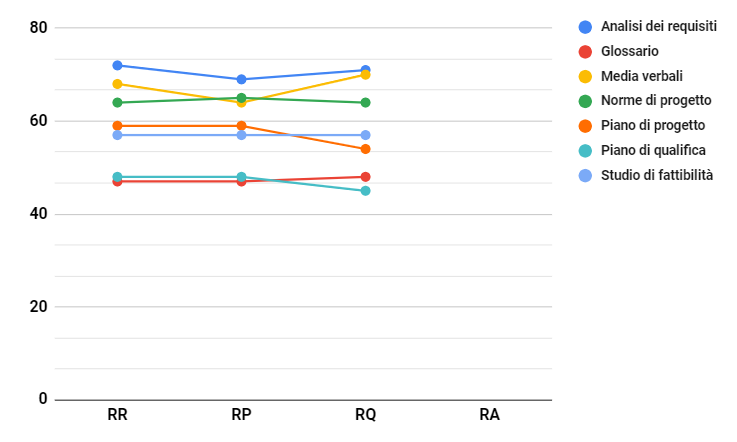
\includegraphics[width=12cm]{images/gulpease.png}
	\caption{Indice di gulpease per revisione}
\end{figure}
\begin{figure}[H]
	\centering
	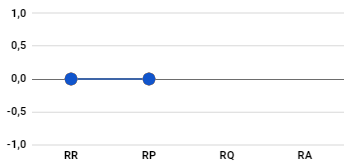
\includegraphics[width=9cm]{images/err_ortografici.png}
	\caption{Errori ortografici per revisione}
\end{figure}

\subsection{MP01 - Schedule Variance}
A causa dei rischi incontrati, il gruppo risulta in ritardo rispetto alla schedulazione delle attività di progetto pianificate.
\begin{figure}[H]
	\centering
	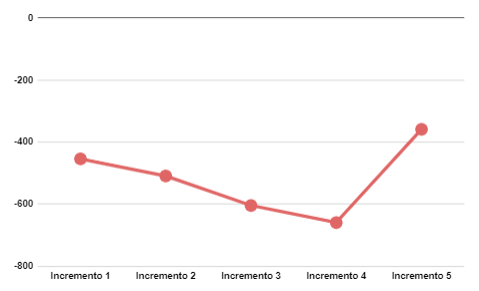
\includegraphics[width=11cm]{images/schedule_variance.png}
	\caption{Andamento metrica Schedule Variance}
\end{figure}

\subsection{MP04 - Cost Variance}

\begin{figure}[H]
	\centering
	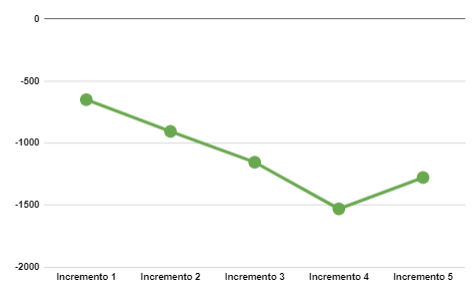
\includegraphics[width=11cm]{images/cost_variance.png}
	\caption{Andamento metrica Cost Variance}
\end{figure}

\subsection{MP06 - Budget Variance}
La seguente metrica verrà tracciata per verificare se alla data corrente si è speso di più o di meno rispetto a quanto previsto.
Se è $>$ 0 significa che il progetto sta spendendo il proprio budget con minor velocità di quanto pianificato, viceversa se negativo.
\begin{figure}[H]
	\centering
	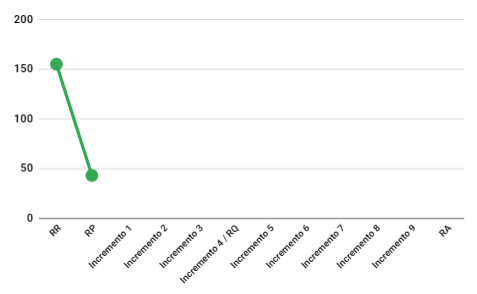
\includegraphics[width=11cm]{images/budget_variance.png}
	\caption{Andamento metrica Budget Variance}
\end{figure}

\subsection{MP07 - Unbudgeted Risks}
Data la possibilità di incontrare rischi, non preventivati in fase di analisi, di seguito verranno illustrate tali evenienze per ogni revisione del progetto:
\begin{figure}[H]
	\centering
	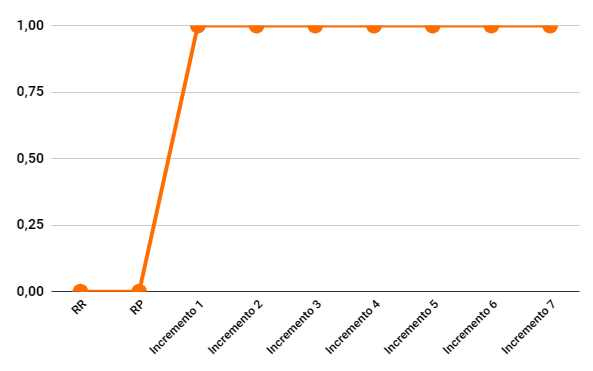
\includegraphics[width=11cm]{images/unbudgeted_risks.png}
	\caption{Andamento metrica Unbudgeted risks}
\end{figure}





